\documentclass{article}
\usepackage{ctex}
\usepackage{graphicx} % 使用graphicx宏包和"\includegraphics[options]{name}"命令插入图片
\usepackage{subcaption} % 使用subcaption宏包来创建subfigure环境,在figure环境中嵌套多图
% \usepackage{subfig} % 使用subfig宏包提供的"\subfloat[sub-caption]{body}"命令,在figure环境中嵌套多图
%! 注意,subcaption宏包和subfig宏包只能加载其中一个,否则编译会报错
\usepackage{wrapfig} % 使用wrapfig宏包进行图文混排
\usepackage[section]{placeins} % 重新定义了"\section{}"命令,在此之前加上了"\Float-Barrrier"命令,阻止浮动体跨过该位置
\usepackage[colorlinks = true,linkcolor=blue]{hyperref}

%* 以下插入的图片外面都套有一层"\fbox{text}"命令,以清楚显示图片的边框界限

\begin{document}

\tableofcontents

\newpage

\section{图片参数}
\subsection{图片原始大小}
% graphicx宏包命令
    %picture in the same file as Tex
    \fbox{\includegraphics{doraemon1.jpg}}
    % XeLaTeX支持pdf、eps、png与jpg图片扩展名,所以可以写带扩展名的图片名称,也可以写不带扩展名的名称,如果不给出扩展名,将按上述4个扩展名的顺序依次搜索文件(吴康隆P50)

%* 通过图片的相对路径引用图片
    \includegraphics{../LaTeX_Picture/doraemon1.jpg} 
    %! 注意,使用相对路径的几个要点:
    %! (1)以"../"符号表示省略的上级路径,在Windows系统中也使用正斜杠
    %! (2)相对路径开始的第一级是".tex"后缀文件所在的文件名,不能比这一级高,当然也不能比这一级低

%* 通过一个专门存放图片的文件夹的路径引用图片
    % reserved file for pictures
    \graphicspath{{../LaTeX_Picture/Reserved file for pictures}}
    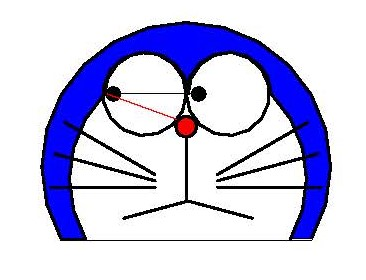
\includegraphics{doraemon2.jpg}
    %!注意,使用"\graphicspath{dir-list}"命令时,路径两边应该套用两层大括号,否则无法成功编译

\subsection{scale表示图片缩放倍数(0.3倍/0.5倍/0.7倍)}
    \fbox{\includegraphics[scale=.3]{doraemon1.jpg}}
    \fbox{\includegraphics[scale=.5]{doraemon1.jpg}}
    \fbox{\includegraphics[scale=.7]{doraemon1.jpg}}

\subsection{width表示图片宽度(3cm/0.3倍文本宽度)}

    \fbox{\includegraphics[width=3cm]{doraemon1.jpg}}
    \fbox{\includegraphics[width=.3\textwidth]{doraemon1.jpg}}

\subsection{height表示图片高度(1cm/0.1倍页高)}
    % 旋转的图片基线会变化,故一般用totalheight代替height(吴康隆P50)
    \fbox{\includegraphics[height=1cm]{doraemon1.jpg}}
    \fbox{\includegraphics[height=.1\textheight]{doraemon1.jpg}}

\subsection{angle表示图片逆时针旋转角度,origin表示图片旋转中心,默认值为l(左),可以设置为r(右)、c(中)、t(顶)、b(底)、B(基线)}
%* 顺时针旋转可以通过在旋转角度前面添加符号来完成
\subsubsection{绕左侧中心逆时针旋转90度}
    \fbox{\includegraphics[angle=90]{doraemon1.jpg}}%counterclockwise
    \fbox{\includegraphics{doraemon1.jpg}}

\subsubsection{绕左侧中心顺时针旋转90度}
    \fbox{\includegraphics[angle=-90]{doraemon1.jpg}}%clockwise
    \fbox{\includegraphics{doraemon1.jpg}}

\subsubsection{绕右侧中心逆时针旋转90度}
    \fbox{\includegraphics{doraemon1.jpg}}
    \fbox{\includegraphics[angle=90, origin=r]{doraemon1.jpg}}

\subsubsection{绕中央中心逆时针旋转90度}
    \fbox{\includegraphics{doraemon1.jpg}}
    \fbox{\includegraphics[angle=90, origin=c]{doraemon1.jpg}}

\subsubsection{绕中心顶端中心逆时针旋转90度}
    \fbox{\includegraphics{doraemon1.jpg}}
    \fbox{\includegraphics[angle=90, origin=t]{doraemon1.jpg}}

\subsubsection{绕底部中心逆时针旋转90度}
    \fbox{\includegraphics{doraemon1.jpg}}
    \fbox{\includegraphics[angle=90, origin=b]{doraemon1.jpg}}

\subsubsection{绕基线中心逆时针旋转90度}
    \fbox{\includegraphics{doraemon1.jpg}}
    \fbox{\includegraphics[angle=90, origin=B]{doraemon1.jpg}}

\subsection{设置图片到边框的距离(原始尺寸/1cm)}
    \fbox{\includegraphics{doraemon1.jpg}}
    {\setlength{\fboxsep}{1cm}
    \fbox{\includegraphics{doraemon1.jpg}}
    }

\section{在文本中插入图片}
\subsection{不使用浮动体环境}
    This is a picture \fbox{\includegraphics{doraemon1.jpg}} inserted into the text.

\subsection{使用浮动体环境}
    This is a picture 
    \begin{figure}[htbp]
        \centering
        \fbox{\includegraphics{doraemon1.jpg}}
        \caption{doraemon\_figure}
    \end{figure}
    independent of the text.
    % 可选参数h、t、b、p分别代表“插入此处”(here)、“插入页面顶部”(top)、“插入页面底部”(bottom)、“允许为浮动体单独开一页”(page),一般将其排列为"htbp",表示插入位置的优先顺序,如果不输入,则默认值为"tbp"
    %rfr 还可以在在可选参数中输入"!"符号,一般将其放置在开头,表示忽略“与浮动放置区域中可容纳的浮动数量或区域最大尺寸相关的任何限制。否则,参数定义的限制适用”,参考:https://ask.latexstudio.net/ask/article/644.html
    %? 标题中的下划线不能直接输入,需要在前面加上反斜杠,另一种输出的办法是在下划线外面套上"\detokenize{}"命令,相当于在前面加反斜杠,书中还介绍了第三种方式,直接在整个标题的外面套上"detokenize{}"命令,即"\caption{\detokenize{doraemon_figure}}",但是经检验,这种输入方式会导致编译报错,而如果将"\caption{}"命令中的参数放置到正文中,就可以成功编译,暂时不知道原因是什么。

\section{图文混排}
% wrapfig宏包命令
    Texte texte texte texte texte texte texte
    texte texte texte texte texte texte texte
    texte texte texte texte texte texte...
    Texte texte texte texte texte texte texte
    texte texte texte texte texte texte texte
    texte texte texte texte texte texte...

    \begin{wrapfigure}{l}{5cm}%Notice that this is the argument of width
        \centering
        \fbox{\includegraphics{doraemon1.jpg}}
        \caption{doraemon\_wrapfigure}
    \end{wrapfigure}

    Texte texte texte texte texte texte texte
    texte texte texte texte texte texte texte
    texte texte texte texte texte texte...
    Texte texte texte texte texte texte texte
    texte texte texte texte texte texte texte
    texte texte texte texte texte texte...
    Texte texte texte texte texte texte texte
    texte texte texte texte texte texte texte
    texte texte texte texte texte texte...
    Texte texte texte texte texte texte texte
    texte texte texte texte texte texte texte
    texte texte texte texte texte texte...
    % wrapfigure环境有两个必选参数,两个可选参数:[linenum]{place}[overhang]{picwidth},必选参数包括{place}和{picwidth},{place}可以选择r、l、i、o,分别代表图片在文字段的左侧、右侧、近书脊、远书脊,{picwidth}代表图片的宽度,图片的高度会自动调整;可选参数包括[linenum]和[overhang],[linenum]代表图片所占行数,一般不指定,[overhang]代表允许图片超出页面文本区的宽度,默认是0pt,即不允许图片超出页面文本区,该项可以使用"\width"代替图片的宽度,填入"\width"将允许把图片全部放入页边区域(吴康隆P51)

\section{并排插入图片}
%rfr 可以参考:https://liam.page/2018/01/11/floats-in-LaTeX-multiple-elements-in-a-single-float/、https://blog.csdn.net/yzy_1996/article/details/117574086、https://blog.csdn.net/Infinity_07/article/details/122796312
\subsection{并排插入共享标题的图片}
    使用\LaTeX 原生命令中的figure环境和graphicx宏包提供的``\textbackslash includegraphics[options]\{name\}''就可以完成简单的并排图片的插入,一般会在可选参数中设置width为文本宽度的倍数,如果不设置可选参数,则会将图片按照原始大小排列在一起,但是这很可能导致因为图片总宽度超过文本宽度而无法在一行上并排放置,下面展示不设置可选参数(\ref{1})和在可选参数中设置width为0.25倍文本宽度(\ref{2})两种情况的打印效果。
    %* 在可选参数中设置width而非其他特征,比如height、scale等,原因也很好理解,因为width可以通过设置为当前文本宽度的倍数来进行调整,而当前文本宽度的值是确定的,这样,可以最方便地调整图片在文本中的大小比例,而其他图片的特征都缺少这样一个确定的基准值,因此通常不怎么用到

    \begin{figure}[htbp]
        \centering
        \fbox{\includegraphics{doraemon1.jpg}}
        \fbox{\includegraphics{doraemon1.jpg}}
        \fbox{\includegraphics{doraemon1.jpg}}
        \caption{doraemon\_figure\_graphicx\_horizontal (1)}
        \label{1}
    \end{figure}

    \begin{figure}[htbp]
        \centering
        \fbox{\includegraphics[width=.25\textwidth]{doraemon1.jpg}}
        \fbox{\includegraphics[width=.25\textwidth]{doraemon1.jpg}}
        \fbox{\includegraphics[width=.25\textwidth]{doraemon1.jpg}}
        \caption{doraemon\_figure\_graphicx\_horizontal (2)}
        \label{2}
    \end{figure}

    在``\textbackslash includegraphics[options]\{name\}''命令之间插入``\textbackslash hfill''命令,可以使两侧的图片分别位于文本的左右边界(\ref{3}),并且均匀调整水平方向上图片之间的距离。

    \begin{figure}[htbp]
        \centering
        \fbox{\includegraphics[width=.25\textwidth]{doraemon1.jpg}}
        \hfill
        \fbox{\includegraphics[width=.25\textwidth]{doraemon1.jpg}}
        \hfill
        \fbox{\includegraphics[width=.25\textwidth]{doraemon1.jpg}}
        \caption{doraemon\_figure\_graphicx\_horizontal (3)}
        \label{3}
    \end{figure}

    如果在``\textbackslash includegraphics[options]\{name\}''命令之间插入``\textbackslash\textbackslash''符号,就可以达到像表格中一样的换行效果,使图片纵向排列(\ref{4})。

    \begin{figure}[htbp]
        \centering
        \fbox{\includegraphics[width=.25\textwidth]{doraemon1.jpg}}\\
        \fbox{\includegraphics[width=.25\textwidth]{doraemon1.jpg}}\\
        \fbox{\includegraphics[width=.25\textwidth]{doraemon1.jpg}}
        \caption{doraemon\_figure\_graphicx\_vertical (1)}
        \label{4}
    \end{figure}

    还可以在``\textbackslash\textbackslash''符号的后面加上用中括号括起来的距离长度,比如``[2ex]'',来增加图片之间的距离(\ref{5})。

    \begin{figure}[htbp]
        \centering
        \fbox{\includegraphics[width=.25\textwidth]{doraemon1.jpg}}\\[2ex]
        \fbox{\includegraphics[width=.25\textwidth]{doraemon1.jpg}}\\[2ex]
        \fbox{\includegraphics[width=.25\textwidth]{doraemon1.jpg}}
        \caption{doraemon\_figure\_graphicx\_vertical (2)}
        \label{5}
    \end{figure}

\subsection{并排插入拥有小标题的图片}
    但是上述这种设置方式没有办法为每个小图设置小标题\footnote{情况其实有些复杂,应该分成两种情况来讨论:如果是并排插入图片,在每一条``\textbackslash includegraphics[options]\{name\}''命令之后插入``\textbackslash caption\{\}''命令,编译不会报错,但是会导致最后带标题的图片变成纵向排列;如果是纵向插入图片,在每一条``\textbackslash includegraphics[options]\{name\}''命令之后,``\textbackslash\textbackslash''符号之前插入``\textbackslash caption\{\}''命令,编译会报错。},此时使用minipage环境将每个小图包起来,就可以在各自的minipage环境中通过``\textbackslash caption\{\}''命令设置小标题(\ref{6})。注意,minipage环境需要设置表示边框宽度的必选参数(通常就是需要设置的图片的宽度),否则编译会报错。相应地,原来``\textbackslash includegraphics[options]\{name\}''命令的可选参数中的width的值应该增大,因为此时该命令放置在minipage环境中,可选参数表示的不再是原来文本宽度的倍数,而是minipage环境中文本宽度的倍数,一般改为单倍的文本宽度。

    \begin{figure}[htbp]
        \centering
        \fbox{
            \begin{minipage}{.25\textwidth}
                \fbox{\includegraphics[width=\textwidth]{doraemon1.jpg}}
                \caption{doraemon (1)}
            \end{minipage}
        }
        \hfill
        \fbox{
            \begin{minipage}{.25\textwidth}
                \fbox{\includegraphics[width=\textwidth]{doraemon1.jpg}}
                \caption{doraemon (2)}
            \end{minipage}
        }
        \hfill
        \fbox{
            \begin{minipage}{.25\textwidth}
                \fbox{\includegraphics[width=\textwidth]{doraemon1.jpg}}
                \caption{doraemon (3)}
            \end{minipage}
        }
        \caption{doraemon\_minipage\_caption}
        \label{6}
    \end{figure}

\subsection{并排插入拥有子编号的图片}
    上述这种设置方式会导致小图的编号接着前面大图的编号往下继续编号,而没有重新编号。为了让每个并排插入的小图能够拥有自己的子编号,让子编号重新编号,让小图共享的母编号接着前面大图的编号往下继续编号,有两种宏包可以选择。

\subsubsection{subfig宏包}
    subfig宏包的的前身是subfigure宏包,后者现已不再使用。subfig宏包提供了``\textbackslash subfloat[subcaption]\{body\}''命令,其原理类似minipage环境,可选参数用来输入小图标题,必选参数用来输入``\textbackslash includegraphics[options]\{name\}''命令,``\textbackslash subfloat[subcaption]\{body\}''命令没有用来控制图片宽度的参数,图片的宽度通过嵌套在其中的``\textbackslash includegraphics[options]\{name\}''命令来控制(\ref{7})。

%todo subfig宏包命令,和subcaption宏包不兼容
%rfr 可以到文件"Picture_subfig.tex"中查看相应的效果
    % \begin{figure}[htbp]
    %     \centering
    %     \fbox{
    %         \subfloat[doraemon (1)\label{7.1}]{

    %             \fbox{\includegraphics[width=.25\textwidth]{doraemon1.jpg}}
    %         }
    %     }
    %     \hfill
    %     \fbox{
    %         \subfloat[doraemon (2)\label{7.2}]{

    %             \fbox{\includegraphics[width=.25\textwidth]{doraemon1.jpg}}
    %         }
    %     }
    %     \hfill
    %     \fbox{
    %         \subfloat[doraemon (3)]{
    %             \label{7.3} %* "\label{}"命令既可以放在可选参数内,也可以放在必选参数内
    %             \fbox{\includegraphics[width=.25\textwidth]{doraemon1.jpg}}
    %         }
    %     }
    %     \caption{doraemon\_subfig\_subfloat}
    %     \label{7}
    % \end{figure}

\subsubsection{subcaption宏包}
    subcaption宏包提供了三种方式来解决上述问题。第一种方式是通过将表(\label{6})中的``\textbackslash caption\{\}''命令替换为``\textbackslash subcaption\{\}''命令,就可以使小图重新编号(\ref{8})。

%todo subcaption宏包命令,和subfig宏包不兼容 
    \begin{figure}[htbp]
    \centering
    \fbox{
        \begin{minipage}{.25\textwidth}
            \fbox{\includegraphics[width=\textwidth]{doraemon1.jpg}}
            \subcaption{doraemon (1)}
        \end{minipage}
    }
    \hfill
    \fbox{
        \begin{minipage}{.25\textwidth}
            \fbox{\includegraphics[width=\textwidth]{doraemon1.jpg}}
            \subcaption{doraemon (2)}
        \end{minipage}
    }
    \hfill
    \fbox{
        \begin{minipage}{.25\textwidth}
            \fbox{\includegraphics[width=\textwidth]{doraemon1.jpg}}
            \subcaption{doraemon (3)}
        \end{minipage}
    }
    \caption{doraemon\_minipage\_subcaption}
    \label{8}
    \end{figure}

    第二种方式是通过``\textbackslash subcaptionbox\{heading\}[width]\{content\}''命令来完成,其原理类似minipage环境,第一个必选参数用来输入小图标题(而在``\textbackslash subfloat[subcaption]\{body\}''命令中这是一个可选参数),第二个可选参数用来输入边框的宽度,第三个必选参数用来输入``\textbackslash includegraphics[options]\{name\}''命令。注意,和在minipage环境中不同,``\textbackslash includegraphics[options]\{name\}''命令中表示图片宽度的可选参数在``\textbackslash subcaptionbox\{heading\}[width]\{content\}''命令中仍然是以文本宽度作为基准的,因此不需要改变其大小。另外,根据subcaption宏包的官方手册显示,``\textbackslash subcaptionbox\{heading\}[width]\{content\}''的第二个可选参数表示的是边框的宽度,默认值就是其中图片的宽度,但是经检验,将其设置为图片宽度(\ref{9})和不设置这一可选参数(\ref{10})两种情况下,前者得到的效果是有略微差异的,前者和使用``\textbackslash subcaption\{\}''命令(\ref{8})的效果相同,后者和使用``\textbackslash subfloat[subcaption]\{body\}''命令(\ref{7})的效果相同。

%todo subcaption宏包命令,和subfig宏包不兼容
    \begin{figure}[htbp]
        \fbox{
            \subcaptionbox{doraemon (1)}[.25\textwidth]{
                \fbox{\includegraphics[width=.25\textwidth]{doraemon1.jpg}}}
        }
        \hfill
        \fbox{
            \subcaptionbox{doraemon (2)}[.25\textwidth]{
                \fbox{\includegraphics[width=.25\textwidth]{doraemon1.jpg}}}
        }
        \hfill
        \fbox{
            \subcaptionbox{doraemon (3)}[.25\textwidth]{
                \fbox{\includegraphics[width=.25\textwidth]{doraemon1.jpg}}}
        }
        \caption{doraemon\_subcaptionbox (1)}
        \label{9}
    \end{figure}

%todo subcaption宏包命令,和subfig宏包不兼容
    \begin{figure}[htbp]
        \fbox{
            \subcaptionbox{doraemon (1)}{
                \fbox{\includegraphics[width=.25\textwidth]{doraemon1.jpg}}}
        }
        \hfill
        \fbox{
            \subcaptionbox{doraemon (2)}{
                \fbox{\includegraphics[width=.25\textwidth]{doraemon1.jpg}}}
        }
        \hfill
        \fbox{
            \subcaptionbox{doraemon (3)}{
                \fbox{\includegraphics[width=.25\textwidth]{doraemon1.jpg}}}
        }
        \caption{doraemon\_subcaptionbox (2)}
        \label{10}
    \end{figure}

    第三种方式是通过subfigure环境(注意,该环境并非来自已经不再使用的subfigure宏包)来完成,其原理和minipage环境几乎完全相同,同样需要输入代表边框宽度的必选参数,并且其中``\textbackslash includegraphics[options]\{name\}''命令的可选参数表示的宽度需要增大,因为此时``\textbackslash textwidth''代表的文本宽度变成了subfigure创建的边框中的文本宽度,一般改为单倍的文本宽度。另外还有一点有意思的是,在subfigure中不管使用``\textbackslash caption\{\}''命令还是``\textbackslash subcaption\{\}''命令,小图都会重新编号,效果没有区别(\ref{11})。

%todo subcaption宏包命令,和subfig宏包不兼容
    \begin{figure}[htbp]
        \fbox{
            \begin{subfigure}{.25\textwidth}
                \fbox{\includegraphics[width=\textwidth]{doraemon1.jpg}}
                \subcaption{doraemon (1)}
            \end{subfigure}
        }
        \hfill
        \fbox{
            \begin{subfigure}{.25\textwidth}
                \fbox{\includegraphics[width=\textwidth]{doraemon1.jpg}}
                \subcaption{doraemon (2)}
            \end{subfigure}
        }
        \hfill
        \fbox{
            \begin{subfigure}{.25\textwidth}
                \fbox{\includegraphics[width=\textwidth]{doraemon1.jpg}}
                \caption{doraemon (3)}
            \end{subfigure}
        }
        \hfill
        \caption{doraemon\_subfigure}
        \label{11}
    \end{figure}

\subsection{并排插入不同比例的图片}
    最后还可以讨论一下并排插入不同比例的图片的情况。首先有一个值得注意的现象,那就是在上述命令中,如果在所有图片的``\textbackslash includegraphics[options]\{name\}''命令的可选参数中同时输入width和scale参数,最后会以width参数作为排版的依据,而会忽视设置的scale参数。下面展示通过上面的各种方法设置不同比例图片的排版效果。

    直接通过figure环境和``\textbackslash includegraphics[options]\{name\}''命令(\ref{12})

    \begin{figure}[htbp]
        \centering
        \fbox{\includegraphics[scale=.1]{doraemon1.jpg}}
        \hfill
        \fbox{\includegraphics[scale=.3]{doraemon1.jpg}}
        \hfill
        \fbox{\includegraphics[scale=.5]{doraemon1.jpg}}
        \caption{doraemon\_figure\_graphicx\_scale}
        \label{12}
    \end{figure}

    figure环境嵌套minipage环境,并且使用``\textbackslash caption{}''命令(\ref{13})

    \begin{figure}[htbp]
        \centering
        \fbox{
            \begin{minipage}{.25\textwidth}
                \fbox{\includegraphics[scale=.1]{doraemon1.jpg}}
                \caption{doraemon (1)}
            \end{minipage}
        }
        \hfill
        \fbox{
            \begin{minipage}{.25\textwidth}
                \fbox{\includegraphics[scale=.3]{doraemon1.jpg}}
                \caption{doraemon (2)}
            \end{minipage}
        }
        \hfill
        \fbox{
            \begin{minipage}{.25\textwidth}
                \fbox{\includegraphics[scale=.5]{doraemon1.jpg}}
                \caption{doraemon (3)}
            \end{minipage}
        }
        \caption{doraemon\_minipage\_caption\_scale}
        \label{13}
    \end{figure}

    使用subfig宏包的``\textbackslash subfloat[sub-caption]\{body\}''命令(\ref{14})

%todo subfig宏包命令,和subcaption宏包不兼容 
%rfr 可以到文件"Picture_subfig.tex"中查看相应的效果
    % \begin{figure}[htbp]
    %     \centering
    %     \fbox{
    %         \subfloat[doraemon (1)]{
    %             \fbox{\includegraphics[scale=.1]{doraemon1.jpg}}
    %         }
    %     }
    %     \hfill
    %     \fbox{
    %         \subfloat[doraemon (2)]{
    %             \fbox{\includegraphics[scale=.3]{doraemon1.jpg}}
    %         }
    %     }
    %     \hfill
    %     \fbox{
    %         \subfloat[doraemon (3)]{
    %             \fbox{\includegraphics[scale=.5]{doraemon1.jpg}}
    %         }
    %     }
    %     \caption{doraemon\_subfig\_subfloat\_scale}
    %     \label{14}
    % \end{figure}

    figure环境嵌套minipage环境,并且使用``\textbackslash subcaption{}''命令(\ref{15})

%todo subcaption宏包命令,和subfig宏包不兼容 
    \begin{figure}[htbp]
        \centering
        \fbox{
            \begin{minipage}{.25\textwidth}
                \fbox{\includegraphics[scale=.1]{doraemon1.jpg}}
                \subcaption{doraemon (1)}
            \end{minipage}
        }
        \hfill
        \fbox{
            \begin{minipage}{.25\textwidth}
                \fbox{\includegraphics[scale=.3]{doraemon1.jpg}}
                \subcaption{doraemon (2)}
            \end{minipage}
        }
        \hfill
        \fbox{
            \begin{minipage}{.25\textwidth}
                \fbox{\includegraphics[scale=.5]{doraemon1.jpg}}
                \subcaption{doraemon (3)}
            \end{minipage}
        }
        \caption{doraemon\_minipage\_subcaption\_scale}
        \label{15}
        \end{figure}

    使用subcaption宏包的``\textbackslash subcaptionbox\{heading\}[width]\{content\}''命令(\ref{16}, \ref{17})

%todo subcaption宏包命令,和subfig宏包不兼容
    \begin{figure}[htbp]
        \fbox{
            \subcaptionbox{doraemon (1)}[.25\textwidth]{
                \fbox{\includegraphics[scale=.1]{doraemon1.jpg}}}
        }
        \hfill
        \fbox{
            \subcaptionbox{doraemon (2)}[.25\textwidth]{
                \fbox{\includegraphics[scale=.3]{doraemon1.jpg}}}
        }
        \hfill
        \fbox{
            \subcaptionbox{doraemon (3)}[.25\textwidth]{
                \fbox{\includegraphics[scale=.5]{doraemon1.jpg}}}
        }
        \caption{doraemon\_subcaptionbox\_scale (1)}
        \label{16}
    \end{figure}

%todo subcaption宏包命令,和subfig宏包不兼容
    \begin{figure}[htbp]
        \fbox{
            \subcaptionbox{doraemon (1)}{
                \fbox{\includegraphics[scale=.1]{doraemon1.jpg}}}
        }
        \hfill
        \fbox{
            \subcaptionbox{doraemon (2)}{
                \fbox{\includegraphics[scale=.3]{doraemon1.jpg}}}
        }
        \hfill
        \fbox{
            \subcaptionbox{doraemon (3)}{
                \fbox{\includegraphics[scale=.5]{doraemon1.jpg}}}
        }
        \caption{doraemon\_subcaptionbox\_scale (2)}
        \label{17}
    \end{figure}

    使用subcaption宏包的subfigure环境(\ref{18})

%todo subcaption宏包命令,和subfig宏包不兼容
    \begin{figure}[htbp]
        \fbox{
            \begin{subfigure}{.25\textwidth}
                \fbox{\includegraphics[scale=.1]{doraemon1.jpg}}
                \subcaption{doraemon (1)}
            \end{subfigure}
        }
        \hfill
        \fbox{
            \begin{subfigure}{.25\textwidth}
                \fbox{\includegraphics[scale=.3]{doraemon1.jpg}}
                \subcaption{doraemon (2)}
            \end{subfigure}
        }
        \hfill
        \fbox{
            \begin{subfigure}{.25\textwidth}
                \fbox{\includegraphics[scale=.5]{doraemon1.jpg}}
                \caption{doraemon (3)}
            \end{subfigure}
        }
        \hfill
        \caption{doraemon\_subfigure}
        \label{18}
    \end{figure}

\subsection{结论}
    通过以上各命令的效果,可以发现,排版效果最好的两种方式是:

    \begin{itemize}
        \item 使用subcaption宏包的``\textbackslash subcaptionbox\{heading\}[width]\{content\}''命令,并且为其设置了相等的边框宽度(\ref{16})
        \item 使用subcaption宏包的subfigure环境(\ref{18})
    \end{itemize}
    
    使用minipage环境(\ref{13}, \ref{15})即使设置了相等的边框宽度,也会由于边框的下端没有对齐而导致排版效果不如以上两种方式美观(或许minipage环境有相关参数可以调整这一效果),而使用subfig宏包的``\textbackslash subfloat[sub-caption]\{body\}''命令(\ref{14}),则会由于无法设置图片的宽度,从而和【使用subcaption宏包的``\textbackslash subcaptionbox\{heading\}[width]\{content\}''命令,但是却没有为其设置边框宽度(\ref{17})】一样,导致最后的边框宽度不相等,排版效果最差。
    
    看来,如果要并排插入图片,最好选择使用subcaption宏包的``\textbackslash subcaptionbox\{heading\}[width]\{content\}''命令或者subfigure环境。
    
\clearpage
%rfr 使用"\clearpage"命令来清空浮动队列,并且新开一页,如果此处不使用这一项命令,则"doraemon_subfigure"一图会作为浮动体被插入到下面的文本当中,关于"\newpage"命令和"\clearpage"命令的区别,可以参考:https://blog.csdn.net/weixin_45008608/article/details/115835064、https://www.latexstudio.net/archives/8005.html

\listoffigures
%* 插图目录显示所有在浮动体环境中使用"\caption{heading}"命令对应的图片所在页码
\end{document}